\documentclass{article}

\usepackage{Paper}
\usepackage{tikz}
\renewcommand\theadfont{\bfseries}
\setcellgapes{2pt}

\fancyhead[L]{Maersk Developer}

\geometry{
    a4paper,
    total={170mm, 257mm},   
    left=20mm,
    top=20mm,
    bottom=15mm
}

\pdftitle{Report-Maersk-Developer-CE-SB}

% === TEXT ===
\begin{document}
\thispagestyle{empty}

\vspace*{1.5cm}

\textbf{\huge Report Maersk Developer Oil Rig}\\[.25cm]
{\large Bürli Norman, Frongillo Matteo, Spichtig David}\\[3.5cm]
\begin{center}
    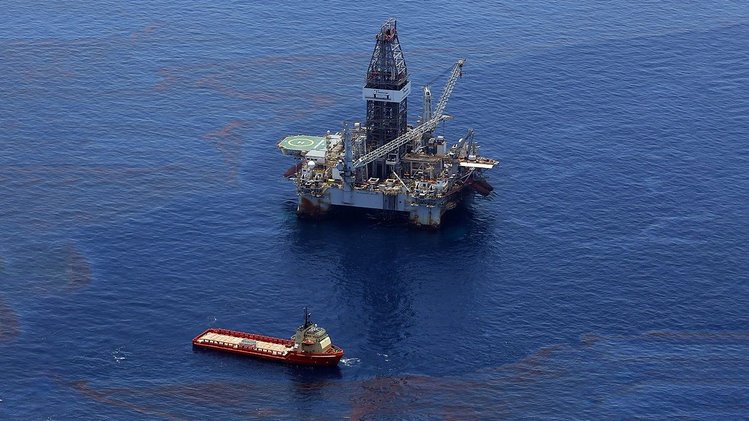
\includegraphics[\lw=.8]{media/main-page.png}\\
\end{center}

\vfill

{\large HS26 -- Corporate Ethics and Sustainability -- Prof. Dr. Claas Wagner}

\newpage
\section*{Question}
\begin{enumerate}
    \item Describe your initial operating strategy, covering the following points:
    \begin{itemize}
        \item Production volume
        \item Overhauls
        \item Maintenance and safety spending
        \item Crew management
    \end{itemize}
\end{enumerate}

\section*{Initial strategy}
The group's initial strategy prioritizes safety while seeking profitable
production, combining planned overhauls, maintenance spending, and crew development.

\subsection*{Production volume}
In practice round 1 (PR1), the production volume was tested by increasing
the production to its maximum (1,650,000 bbls) and hiring more workers.
This allowed the group to understand how extreme conditions affect the sustainability factors.\\
The takeaway for PR1 was that increasing the production volume to
its maximum value was not the correct strategy under the specific starting conditions of PR1,
as profit was reduced by high hiring costs.

In practice round 2 (PR2), the focus shifted from maximizing crude oil
production to testing a more safety-oriented approach.

Decisions in PR1 and PR2 were made to understand how the economic factors
respond to these decisions.

The production volume in Round 1 was set to 1,300,000 bbls. To ensure a
high volume, ten workers were hired. The same strategy was applied
for Round 2.

After Round 1 and Round 2, the group was breaking even.
This result is helpful in identifying the threshold at which production
becomes profitable under specific conditions.

The next steps in production aim to keep the company profitable.

\subsection*{Overhauls}
The overhaul schedule in \autoref{fig:overhauls} illustrates how the
timing of major overhauls affects the BOP (Blow out preventer) value over successive rounds.
\begin{figure}[H]
    \centering
    \resizebox{.9\linewidth}{!}{% Vector recreation of bop_rounds.png; standard TikZ, no shell escape required.
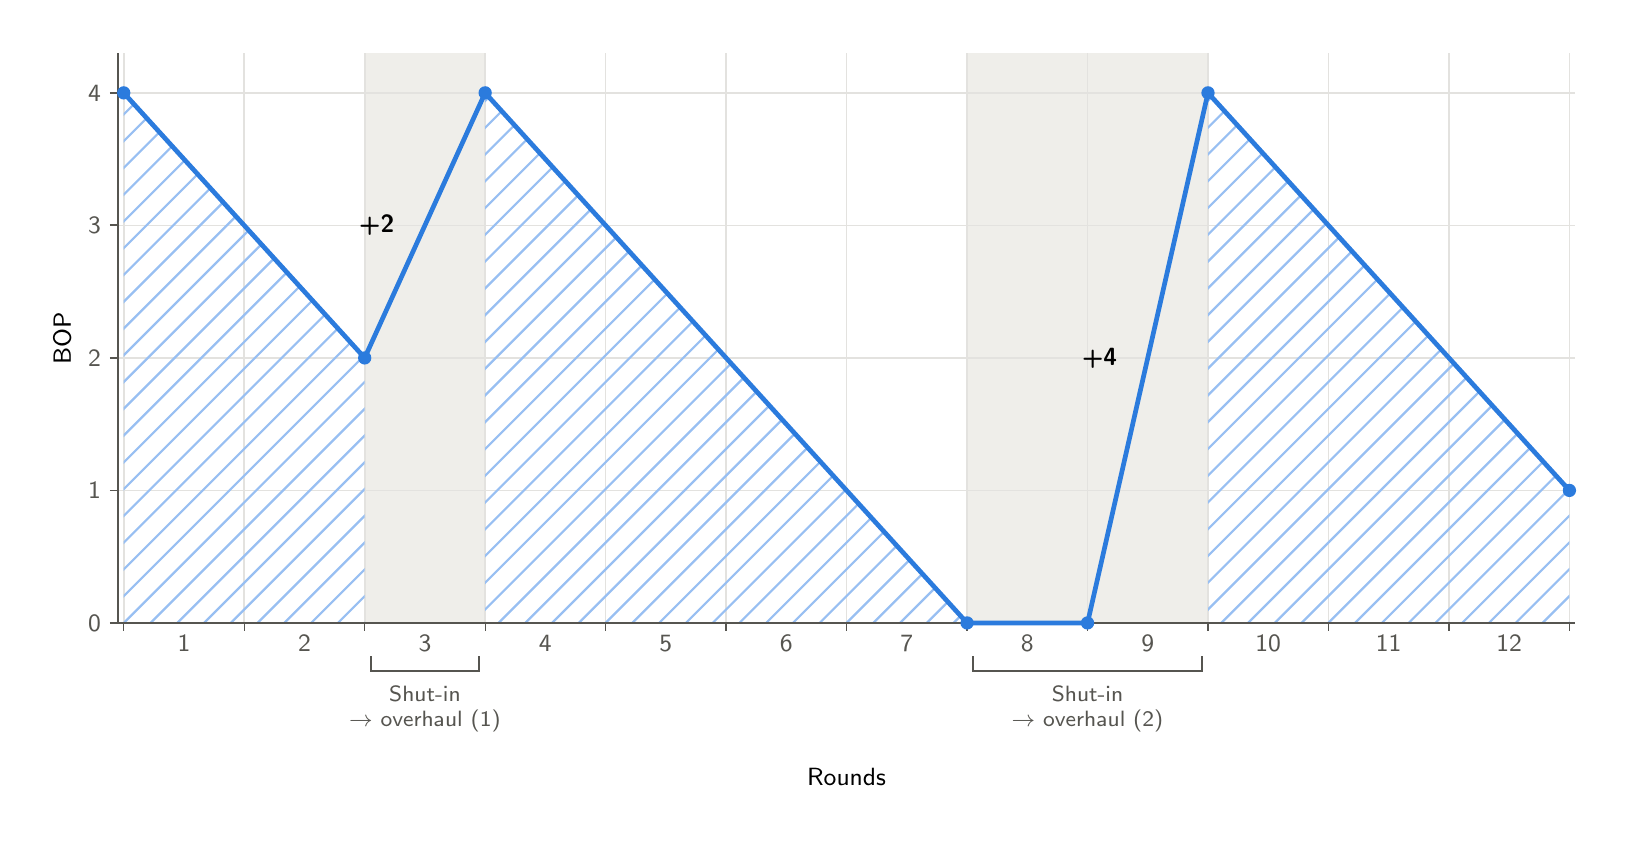
\begin{tikzpicture}[x=1cm,y=1cm,
    font=\sffamily\fontsize{9}{11}\selectfont]
    \definecolor{bopBlue}{HTML}{2B7BDD}
    \definecolor{bopHatch}{HTML}{98BFF2}
    \definecolor{bopGrid}{HTML}{E3E2DF}
    \definecolor{bopShade}{HTML}{EFEEEA}
    \definecolor{bopAxis}{HTML}{565550}
    \path[use as bounding box] (0,0) rectangle (20,10);
    \begin{scope}[shift={(1.22,2.44)},x=1.53cm,y=1.683cm]
        % Shut-in periods: round 3 and rounds 8--9.
        \fill[bopShade] (2,0) rectangle (3,4.3);
        \fill[bopShade] (7,0) rectangle (9,4.3);
        \foreach \x in {0,...,12}
            \draw[bopGrid,line width=.6pt] (\x,0) -- (\x,4.3);
        \foreach \y in {0,...,4}
            \draw[bopGrid,line width=.6pt] (-.05,\y) -- (12.05,\y);

        % Diagonal hatching only beneath the declining BOP segments.
        \begin{scope}
            \clip (0,0) -- (0,4) -- (2,2) -- (2,0) -- cycle
                (3,0) -- (3,4) -- (7,0) -- cycle
                (9,0) -- (9,4) -- (12,1) -- (12,0) -- cycle;
            \foreach \i in {-24,...,60} {
                \pgfmathsetmacro{\hatchStart}{\i*0.2222}
                \draw[bopHatch,line width=.8pt]
                    (\hatchStart,0) -- ++(5,4.5455);
            }
        \end{scope}

        % Axes and ticks; round numbers are centred within each round.
        \draw[bopAxis,line width=.65pt] (-.05,4.3) -- (-.05,0) -- (12.05,0);
        \foreach \y in {0,...,4} {
            \draw[bopAxis,line width=.65pt] (-.115,\y) -- (-.05,\y);
            \node[anchor=east,text=bopAxis,inner sep=0pt]
                at (-.185,\y) {\y};
        }
        \foreach \x in {0,...,12}
            \draw[bopAxis,line width=.45pt] (\x,0) -- (\x,-.06);
        \foreach \round in {1,...,12} {
            \node[anchor=north,text=bopAxis,inner sep=0pt]
                at ({\round-.5},-.09) {\round};
        }

        \draw[bopBlue,line width=1.7pt,line join=round]
            (0,4) -- (2,2) -- (3,4) -- (7,0) -- (8,0) -- (9,4) -- (12,1);
        \foreach \point in {(0,4),(2,2),(3,4),(7,0),(8,0),(9,4),(12,1)}
            \fill[bopBlue] \point circle[radius=2.4pt];
        \node[font=\sffamily\bfseries\fontsize{9}{11}\selectfont]
            at (2.1,3) {+2};
        \node[font=\sffamily\bfseries\fontsize{9}{11}\selectfont]
            at (8.1,2) {+4};

        % Brackets and overhaul annotations below the horizontal axis.
        \draw[bopAxis,line width=.8pt]
            (2.05,-.25) -- (2.05,-.365) -- (2.95,-.365) -- (2.95,-.25);
        \draw[bopAxis,line width=.8pt]
            (7.05,-.25) -- (7.05,-.365) -- (8.95,-.365) -- (8.95,-.25);
        \node[anchor=north,align=center,text=bopAxis,inner sep=0pt,
            font=\sffamily\fontsize{8}{9}\selectfont]
            at (2.5,-.47) {Shut-in\\$\rightarrow$ overhaul (1)};
        \node[anchor=north,align=center,text=bopAxis,inner sep=0pt,
            font=\sffamily\fontsize{8}{9}\selectfont]
            at (8,-.47) {Shut-in\\$\rightarrow$ overhaul (2)};
    \end{scope}
    \node[rotate=90,inner sep=0pt] at (.44,6.05) {BOP};
    \node[inner sep=0pt] at (10.4,.49) {Rounds};
\end{tikzpicture}
}
    \caption{BOP planning schedule}
    \label{fig:overhauls}
\end{figure}

The weather report predicts Beaufort 10 (Storm) in Round 3.
A shut-in is necessary if a storm occurs, as the platform and the oil pumps might
be compromised. An early overhaul is the best option
because it restores the BOP before the expected storm, reducing the risk of a blowout.
Assuming that a Beaufort 10 will occur only in Round 3, this strategy allows
crude oil production to continue for multiple rounds, meaning that major overhauls
would only be needed in Rounds 8 and 9.

The overhaul schedule aims to keep the BOP value above 0. The risk of a blowout
exists regardless of the BOP value, but once it reaches 0, the BOP can no longer
effectively prevent a blowout.

\subsection*{Maintenance and safety spending}
Regular maintenance spending aims to keep the Rig Equipment Condition Index
(RECI) above its baseline value of 100.

Two spending approaches are being considered:
\begin{enumerate}
    \item Invest in maintenance and safety to keep the probability of failures and accidents low\\
    $\to$ Higher spending, lower risk
    \begin{table}[H]
        \centering
        \caption{Maintenance and safety expenditure}
        \begin{tabularx}{0.8\linewidth}{*{4}{>{\centering\arraybackslash}X}}
            \toprule
            & \makecell[c]{\textbf{Maintenance}\\\textbf{[\$/bbl.]}} & \textbf{Safety [\$]} & \textbf{RECI}\\
            \midrule
            \textbf{Baseline} & 8 & 1,200,000 & 100\\
            \textbf{Round 1} & 12 & 2,000,000 & 141\\
            \textbf{Round 2} & 12 & 2,000,000 & 182\\
            \bottomrule
        \end{tabularx}
    \end{table}
    \item Let the RECI degrade and restore it to its baseline value (100) during major overhauls perfomed every six rounds.\\
    $\to$ Cheap but risky. 
\end{enumerate}

During Rounds 1 and 2, the first strategy was used.
To decide which strategy to adopt, a better understanding of the RECI and its effect on safety is needed.

\subsection*{Crew management}
Five crew members were hired in Round 1 to support increased production
while keeping the tiredness index low.

Each round, five crew members receive training, allowing expertise to develop over time while
keeping training costs low.

\section*{Ethical Questions}
\subsection*{\#1: Arctic Investment Opportunity}
The Arctic investment was considered too risky given the expected
return and the high initial cost. Therefore, no investment was made.

\subsection*{\#2: Backup Battery}
The BOP backup battery test costs approximately \$5 million.

\begin{table}[H]
    \centering
    \caption{Cost and probability comparison of a blowout and the BOP backup battery test}
    \label{tab:backup-battery}
    \definecolor{backupBatteryGreen}{HTML}{00B050}
    \renewcommand{\arraystretch}{1.4}
    \setlength{\extrarowheight}{4pt}
    \begin{tabularx}{0.92\linewidth}{>{\raggedright\arraybackslash}X *{3}{>{\centering\arraybackslash}X}}
        \toprule
        & \makecell[c]{\textbf{Cost}\\\textbf{[1e6 \$]}} & \makecell[c]{\textbf{Estimated chance}\\\textbf{[\%]}} & \makecell[c]{\textbf{Normalized cost}\\\textbf{[1e6 \$]}}\\
        \midrule
        \textbf{Blowout (minimum)} & 250 & 1 & 2.5\\
        \makecell[l]{\textbf{Backup Battery}\\\textbf{test of BOP}} & 5 & 100 & \cellcolor{backupBatteryGreen}5\\
        \textbf{Blowout (realistic)} & 500 & 1 & \cellcolor{backupBatteryGreen}5\\
        \bottomrule
    \end{tabularx}
\end{table}


A blowout has an estimated minimum cost of \$250 million, while a
more realistic estimate is \$500 million.
Assuming a 1\% probability of blowout, the expected cost would be
\$5 million, equal to the cost of the test \parenref{tab:backup-battery}.

Under these assumptions, the test costs as much as the estimated expected
loss from a blowout. Carrying out the test is justified as a precaution
to verify the backup system's reliability before relying on it during production.













% \newpage
% \appendix
% \section{Appendix}
% 
% \listoffigures
% 
% \listoftables
% 
% \printbibliography
% 
% \section*{Declarations on the use of AI tools}
% ``\textit{ChatGPT 5.5}'' was used to enhance vocabulary and as a fact-checker.\\
% {\color{darkgray!95}{\textit{All sentences originate from our own ideas and were refined with the support of this tool.}}}\\
% \url{https://chatgpt.com/}
% \thispagestyle{fancy}
\end{document}
